GPU memory use grows strictly linearly with respect to the number of streams and threads. When going from one to two streams, bwa-gasal2 takes twice as much memory. In this section, we will present the case we deemed more representative of real use.

GPU memory (VRAM) use is a delicate topic to assess, since it highly depends on various factors:

\begin{itemize}
	\item the GPU, since the VRAM available may not be sufficient to saturate its computing resources,
	\item the CPU, because how many threads we can instantiate directly impacts how much VRAM we will need,
	\item the RAM, since the sequences also need to be loaded in RAM before being copied to the GPU (although this is rarely a limiting factor, since a given machine has far more RAM than its GPU has VRAM),
	\item and of course, the data set running.
\end{itemize}

We cannot conduct measurements that are corresponding to any algorithmic truth in this case. Consequently we will present the memory use as a case study corresponding to our current machine and data sets, and we will see if, in our example case, the memory use can be deemed as reasonable. We consider the GPU we used (Tesla K40c) with its 2880 CUDA cores and its 12GB or VRAM, as representative of the accelerators generally used.

For this, we start bwa-gasal2 with a substantial low amount of memory, and let the automatic memory extension grow until the end of the program. The memory use for data set SRR150 and SRR250 is shown on figure~\ref{fig:memory-use}. We measured memory use for what we consider a regular use case for our machine : 12 threads, with 2 streams. 

\begin{figure}[h]
	\centering
	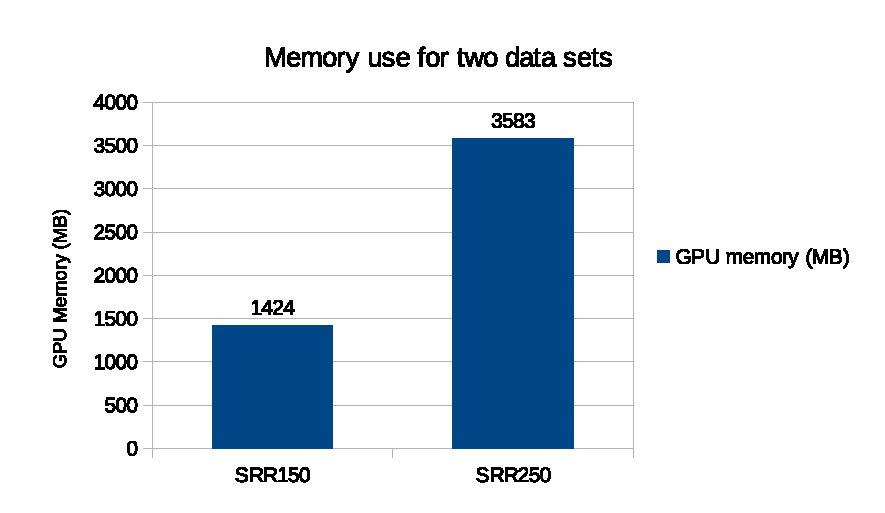
\includegraphics[width=0.9\linewidth]{memory-use}
	\caption{Memory use for our two data sets on our testing machine}
	\label{fig:memory-use}
\end{figure}

On these examples, we need around 1570 MB for a data set with sequences of 150 bases, and 2730 MB for sequences 250 bases long. This shows that our solution will not properly scale with very long sequences, since we will quickly run out of memory for our GPU. Still it is decent for our short-length sequences, where we use less than 1/6th of our total available memory with our worst case scenario. In particular, this allows to use a cheaper accelerator if needed, and in our case, it leaves more memory to accelerate in the future another part of the calculation.
